\section{Array}
\begin{itemize}
    \item Collección de datos del mismo tipo.
    \item En memoria se hace de manera consecutiva.
    \item Con arraylists no se almacena de manera consecutiva.
    \item Elementos:
        \begin{itemize}
            \item Data type: Any valid data type.
            \item Name: How we'll identify.
            \item Size: Maximum numbers of values to hold.
        \end{itemize}
    
    \item En el procesador:
        \begin{itemize}
            \item Tiene una eficiencia mayor.
            \item Como se guarda consecutivamente solo se tiene que buscar una vez en memoria por ser consecutiva.
            \item Por eso se necesita declarar con cuántos elementos inicializar el array.
        \end{itemize}
    
    \item Tener presente cuánto ocupa en memoria cada tipo de elementos.
    \item La función .length recorre todo el array y retorna el número de elementos que tiene.
\end{itemize}


%%%%%%%%%%%%%%%%%%%%%%%%%%%%%%%%%%%%%%%%%%%%%%%%%%%%%%%%%%%%%%%%%%%%%%%%%%%%%%%%%%%%%%%%%%%%%%%%

\subsection{Storing values in the array}
\begin{itemize}
    \item Cuando ingresamos información a un array lo hacemos por orden de índices.
    \item Accesar: por el índice [i].
        \begin{itemize}
            \item System.Out.println(A[i]); // Prints the element stored in that index in memory.
        \end{itemize}
    \item Operations on arrays:
        \begin{itemize}
            \item Deleting elements: cuando se elimina un elemento, se tiene que hacer un corrimiento de las cantidades correspondientes; si por ejemplo tiene que un array de n elementos, se desplaza indices $n$ por los $n + 1$.
            \item A[i] = A[i + 1];
        \end{itemize}
    
    \item Merging arrays:
        \begin{itemize}
            \item array1;
            \item array2; 
            \item merged = array1 + array2; 
        \end{itemize}
    
    \item Passing arrays to functions:
        \begin{enumerate}
            \item Passing entire arrays:
                \begin{itemize}
                    \item Le pasa todo el arreglo, con todo y la posición de memoria.
                \end{itemize}

            \item Passing individual elements: esto permite trabajar el contenido del array por aparte, creo una copia y trabajo con la información, entonces no modifico el array original, si paso la dirección de memoria del índice o de la posición de memoria si voy a alterar el arreglo original.
                \begin{itemize}
                    \item Passing data values 
                    \item Passing addresses 
                \end{itemize}
        \end{enumerate}
\end{itemize}


%%%%%%%%%%%%%%%%%%%%%%%%%%%%%%%%%%%%%%%%%%%%%%%%%%%%%%%%%%%%%%%%%%%%%%%%%%%%%%%%%%%%%%%%%%%%%%%%
\subsection{Caché}
\begin{enumerate}
    \item Almacenamiento 
    \item Temporal 
    \item Fácil Acceso
\end{enumerate}

\subsubsection{Beneficios}
\begin{itemize}
    \item Tener más efectividad.
    \item Reduce el impacto cuando tenemos que interactuar  .
    \item Está enfocado en \textbf{leer}.
\end{itemize}



%%%%%%%%%%%%%%%%%%%%%%%%%%%%%%%%%%%%%%%%%%%%%%%%%%%%%%%%%%%%%%%%%%%%%%%%%%%%%%%%%%%%%%%%%%%%%%%%

\section{Two-Dimensional Array}
\begin{itemize}
    \item Almacena matrices en memoria, tiene varias implicaciones:
        \begin{itemize}
            \item Tener contabilidad de dos indices.
            \item Agregar una línea implica agregar n cantidad de el array anidado.
        \end{itemize}
    
    \item Se almacena de la misma manera que un array de una dimensión.
    \item Cuando se almacena un array bidimensional, se hacen operaciones matemáticas para ubicar en memoria los indices.
    \item Inicialización:
        \begin{itemize}
            \item Se declaran valores al momento de declarar.
            \item Se declaran valores parametrados.
        \end{itemize}
\end{itemize}


%%%%%%%%%%%%%%%%%%%%%%%%%%%%%%%%%%%%%%%%%%%%%%%%%%%%%%%%%%%%%%%%%%%%%%%%%%%%%%%%%%%%%%%%%%%%%%%%

\section{Multi-Dimensional array}
\begin{itemize}
    \item Multidimensional array:
    \begin{itemize}
        \item \emph{\textbf{Ejemplo: }Graficador de imágenes}
            \begin{align*}
                grafo \overbrace{[t_1]}^{\text{  Temporalidad  }}\underbrace{[x_1][y_1]}_{\text{  Cuadrícula  }} & = \underbrace{\text{  Color  }}_{255}\\ 
            \end{align*}
        
        \item Entonces el tiempo puede tener manifestación en un gif, las imágenes que resultan se pintan en la pantalla. Mientras más pixeles tenemos mejor la calidad.
            \begin{figure}[htbp]
                \centering
                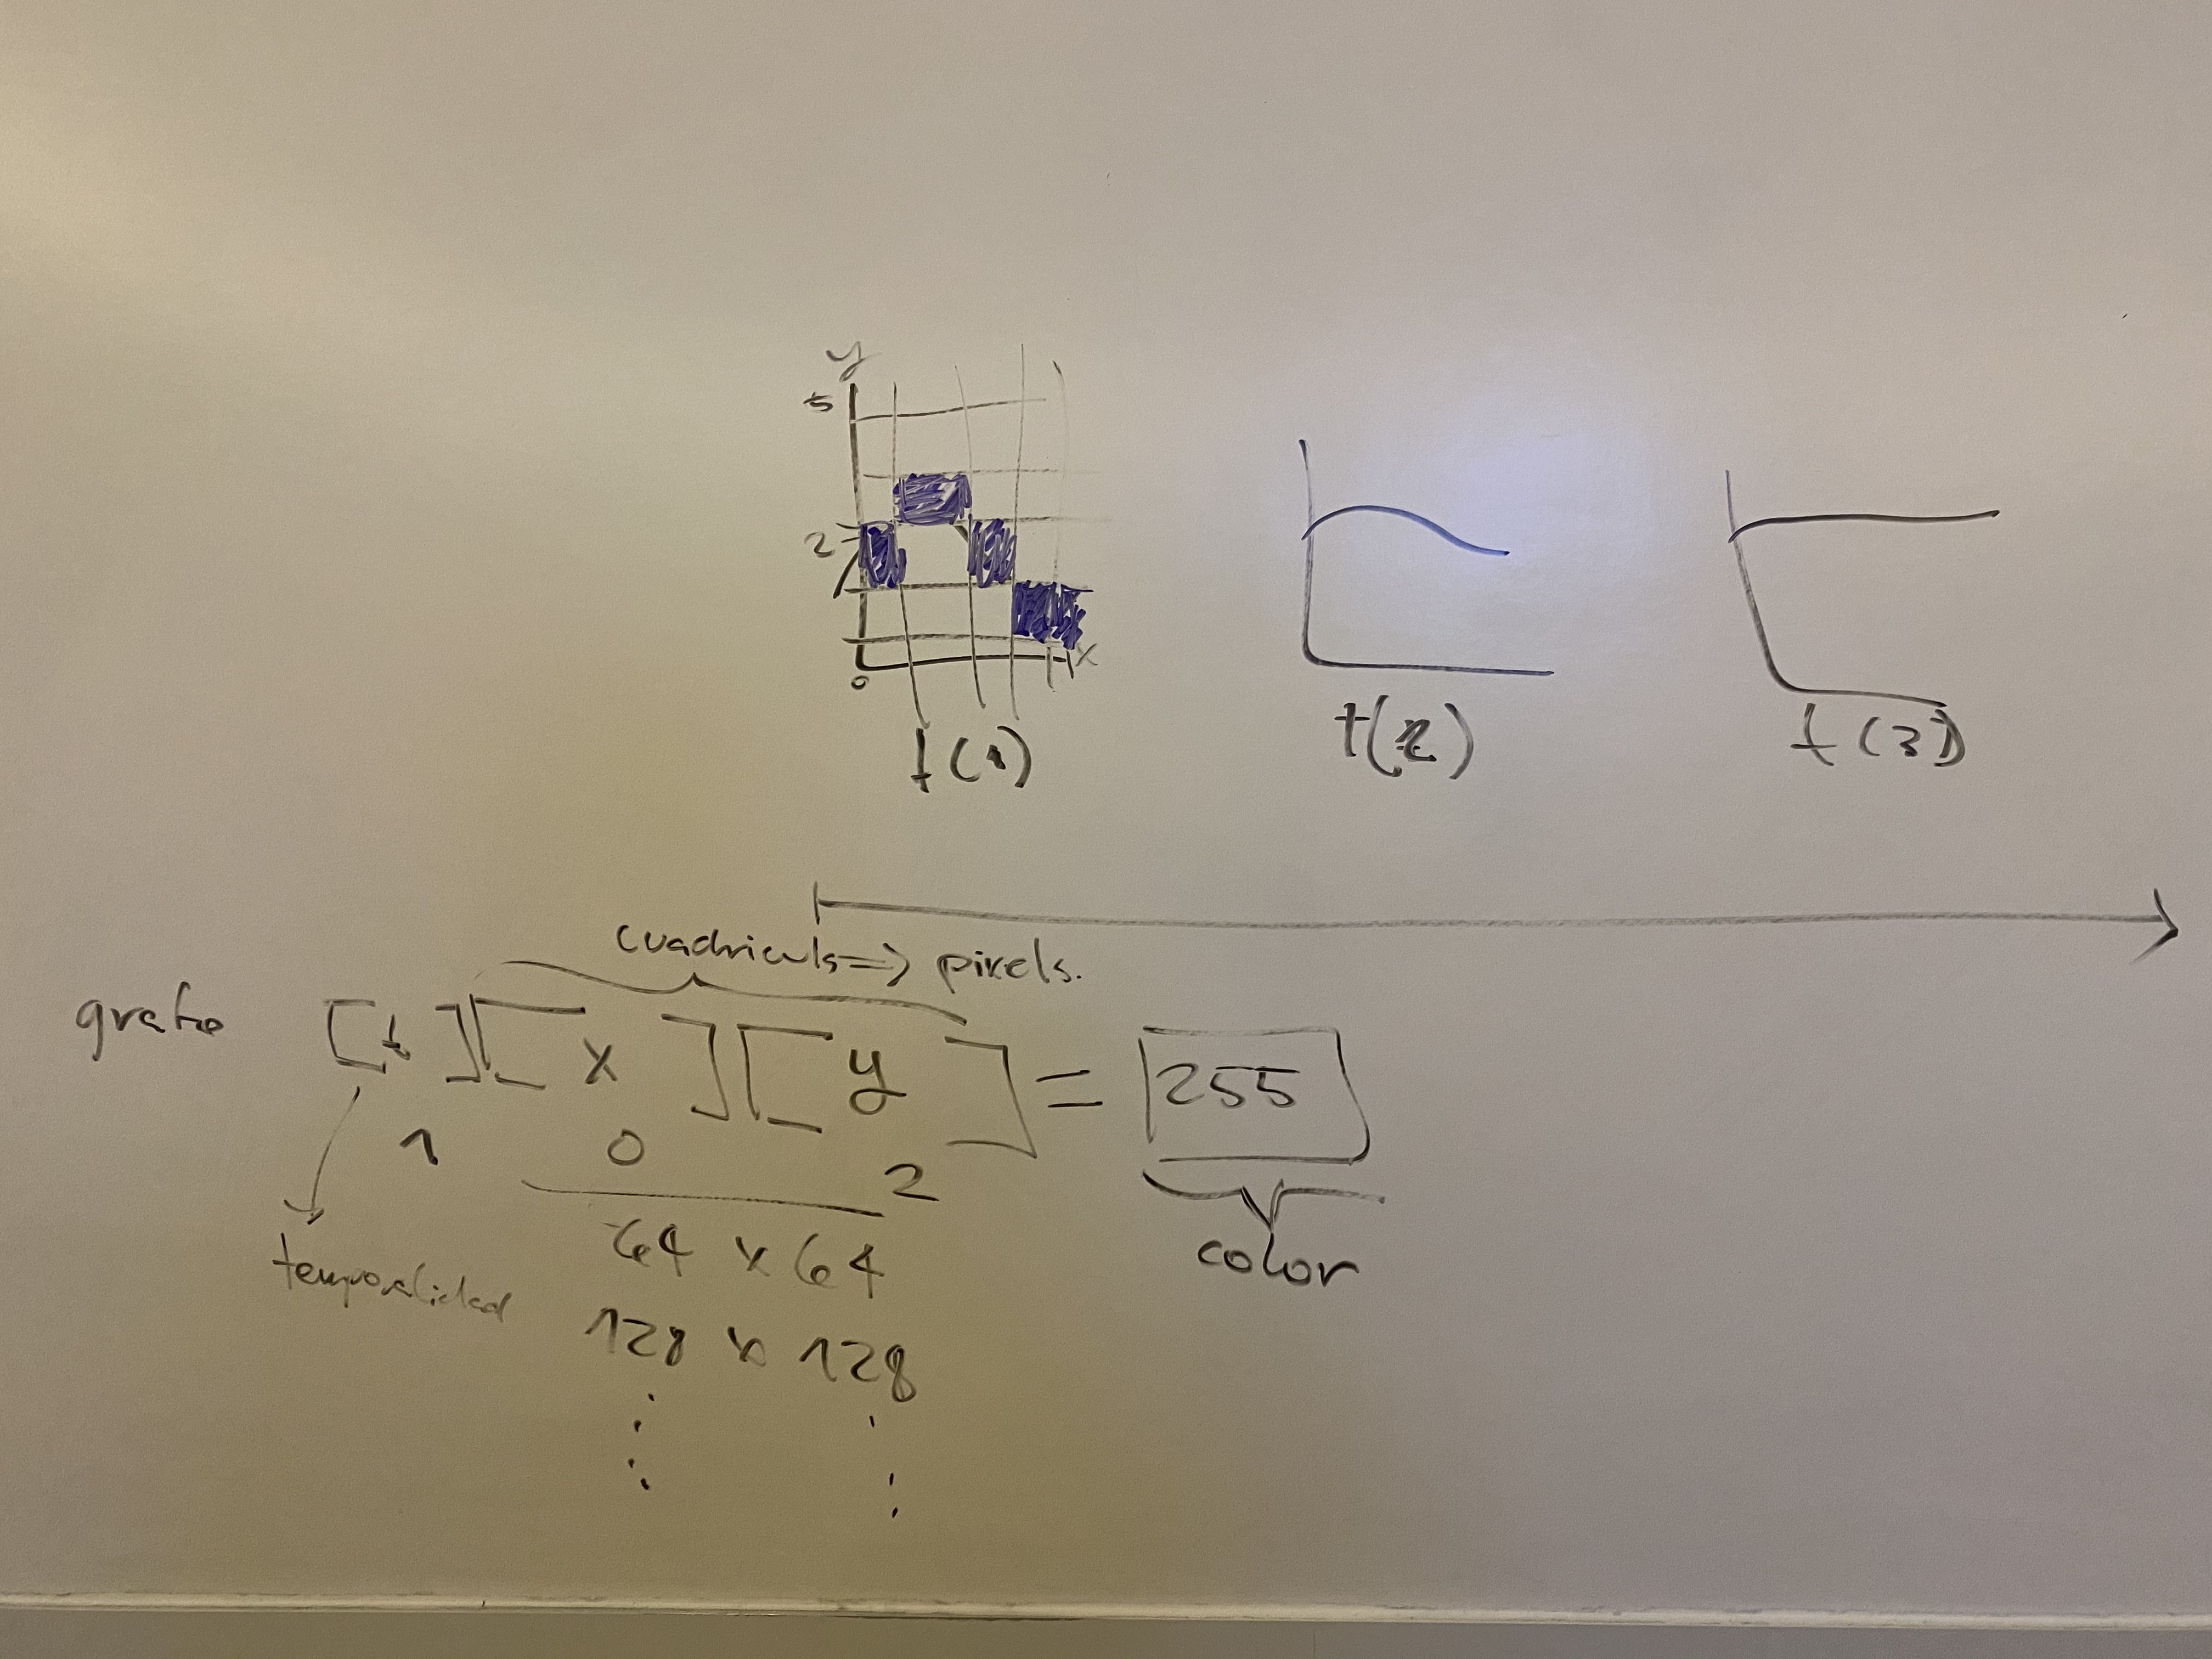
\includegraphics[width=12cm]{./../__Imagenes__/2020-01-27-ED-01.jpeg}
                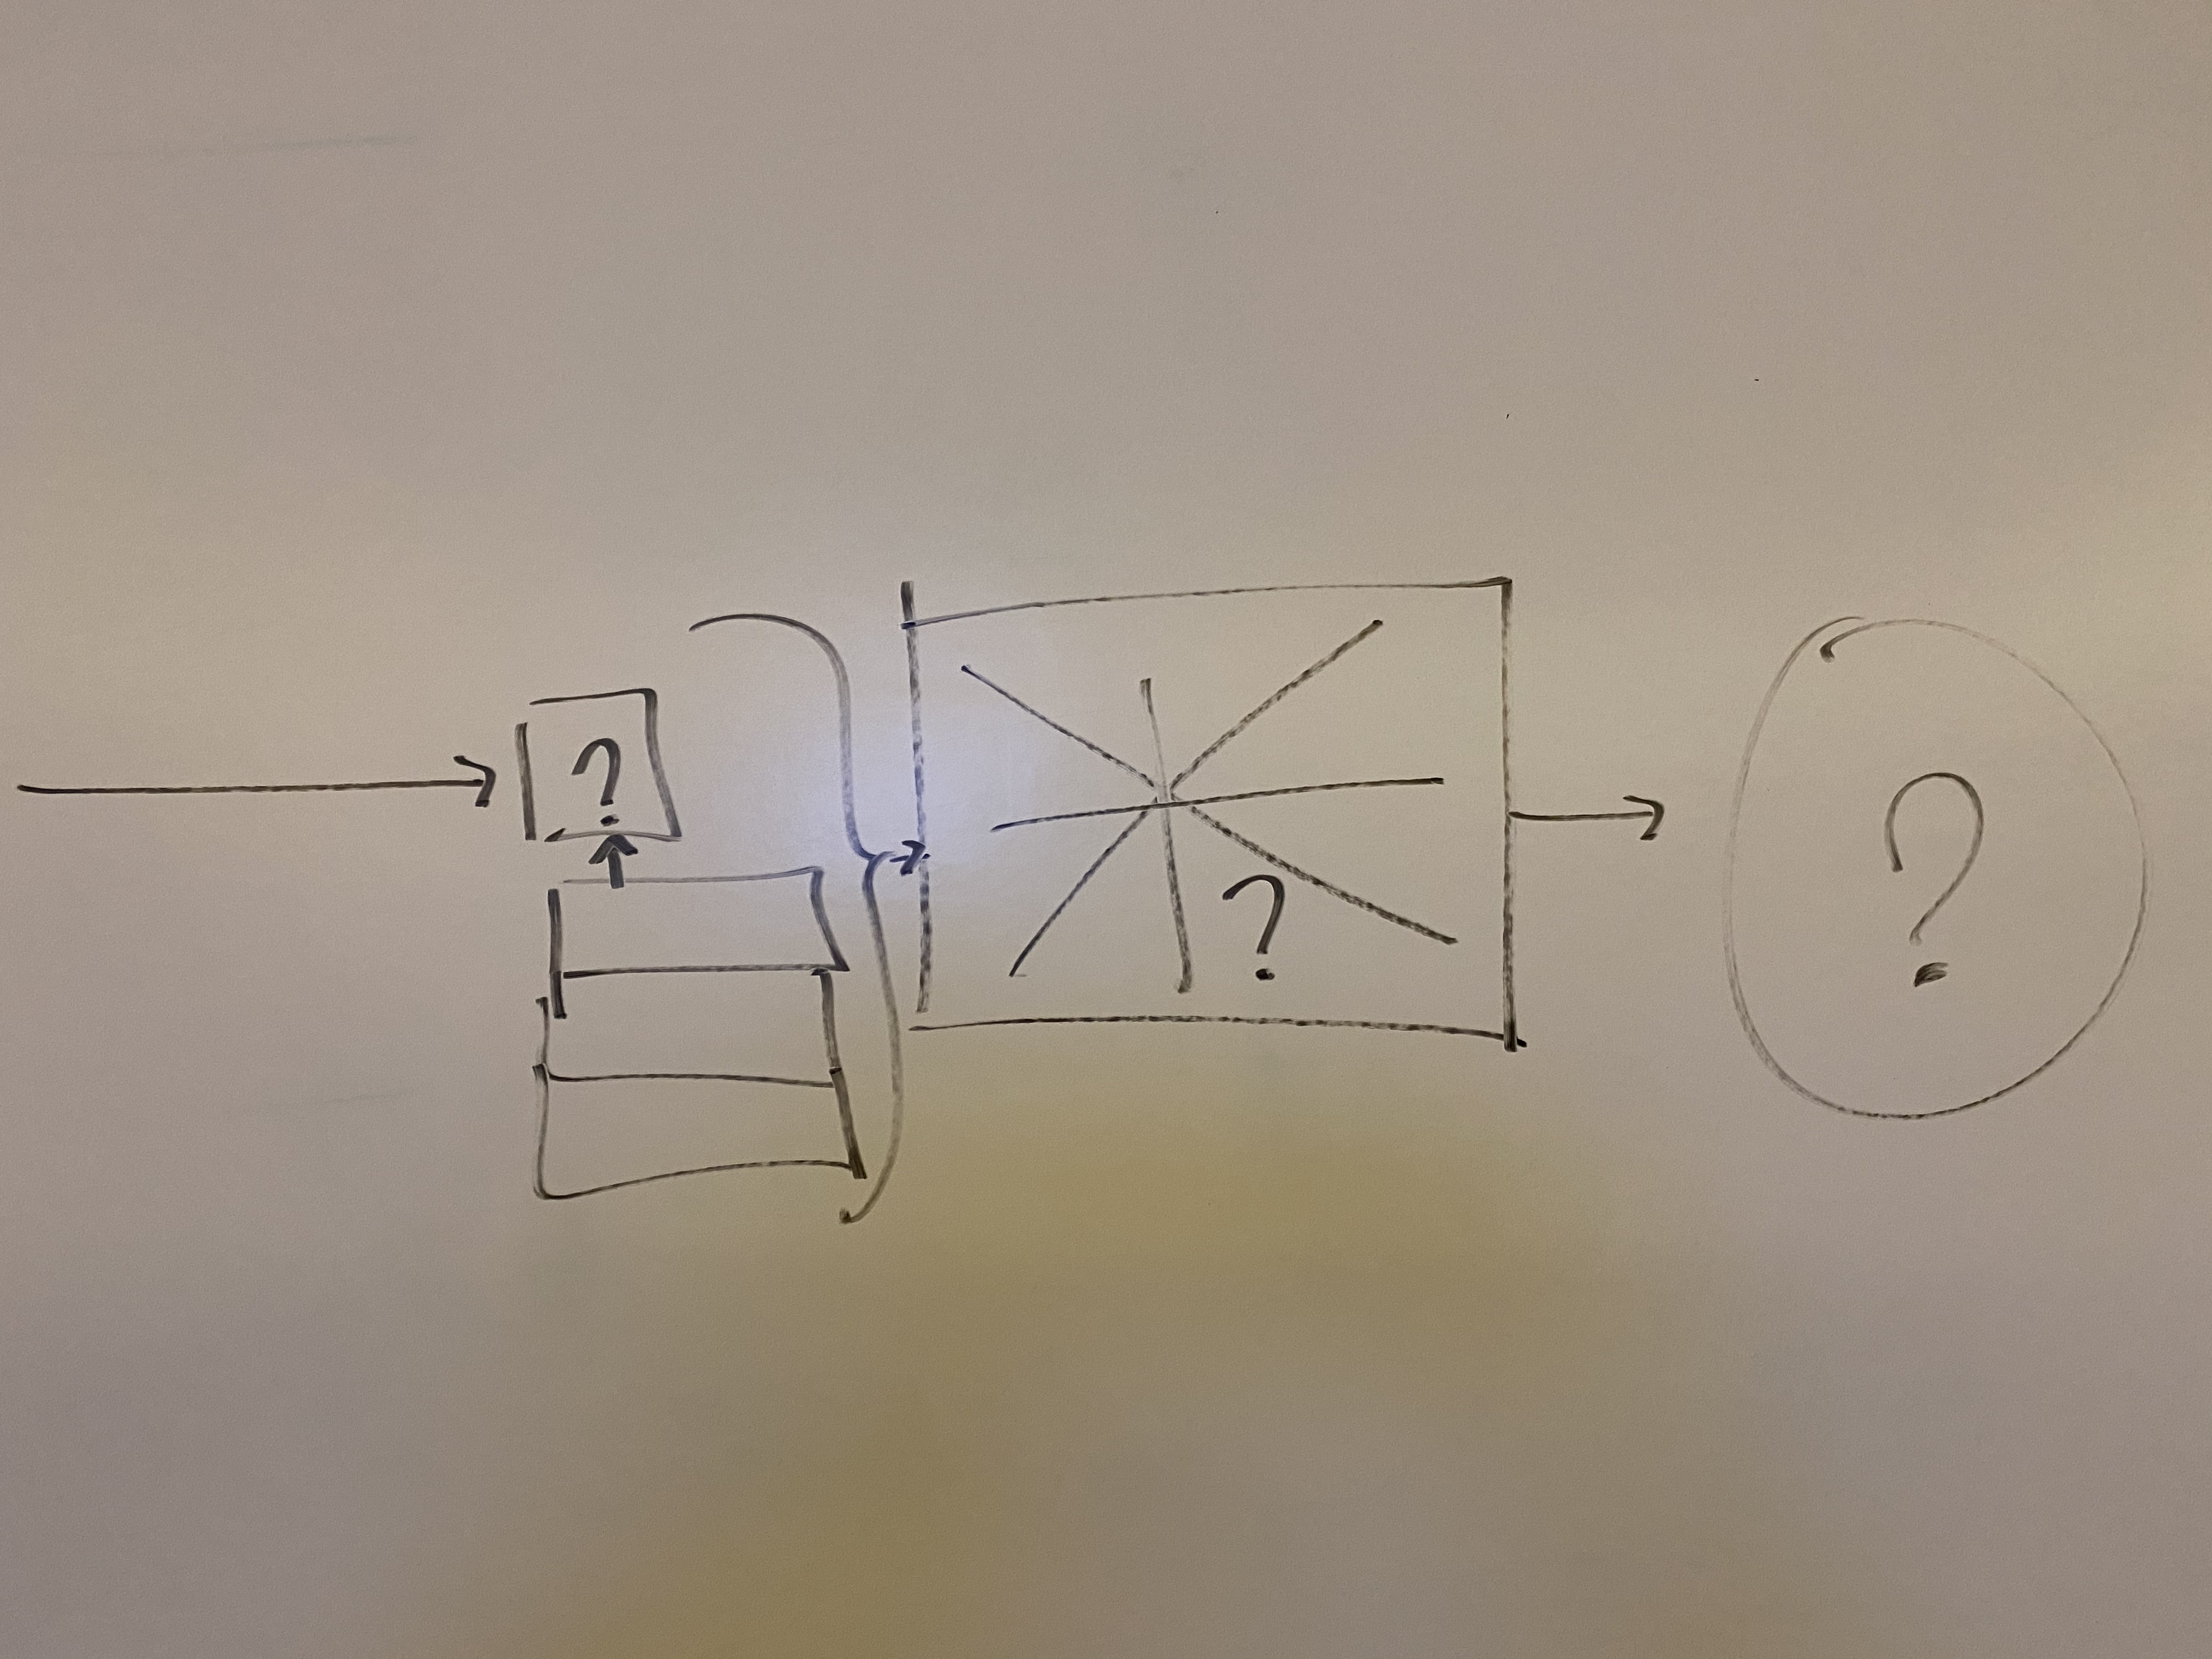
\includegraphics[width=12cm]{./../__Imagenes__/2020-01-27-ED-02.jpeg}
                \caption{Ejemplo de multidimensional arrays \& el black box exercise}
                \label{}
            \end{figure}
    \end{itemize}
    
    \item Los arrays multidimensionales podemos combinarlos con objetos : 
        \begin{itemize}
            \item Nos va permitir más que un solo valor.
            \item Se puede almacenar objetos en el array, por lo general se va a tener que tener el mismo tamaño.
            \item En Java se puede declarar un array de tipos de datos objetos.
        \end{itemize}
\end{itemize}

